\documentclass[10pt]{article}
\usepackage[T1]{fontenc}\usepackage{lmodern}\usepackage[landscape,margin=.45in]{geometry}
\usepackage{tikz,amsmath,xcolor,microtype,hyperref,graphicx}
\usetikzlibrary{arrows.meta,positioning,fit,shapes.geometric}
\hypersetup{pdftitle={Theorem Dependency Graph: Raw Level-2 NMSC Classification},pdfauthor={Alec Kriebel}}
\pagestyle{empty}
\begin{document}
\begin{center}\Large\bfseries Theorem Dependency Graph: Raw Level-2 NMSC Classification\end{center}
\begin{center}\resizebox{.94\linewidth}{!}{%
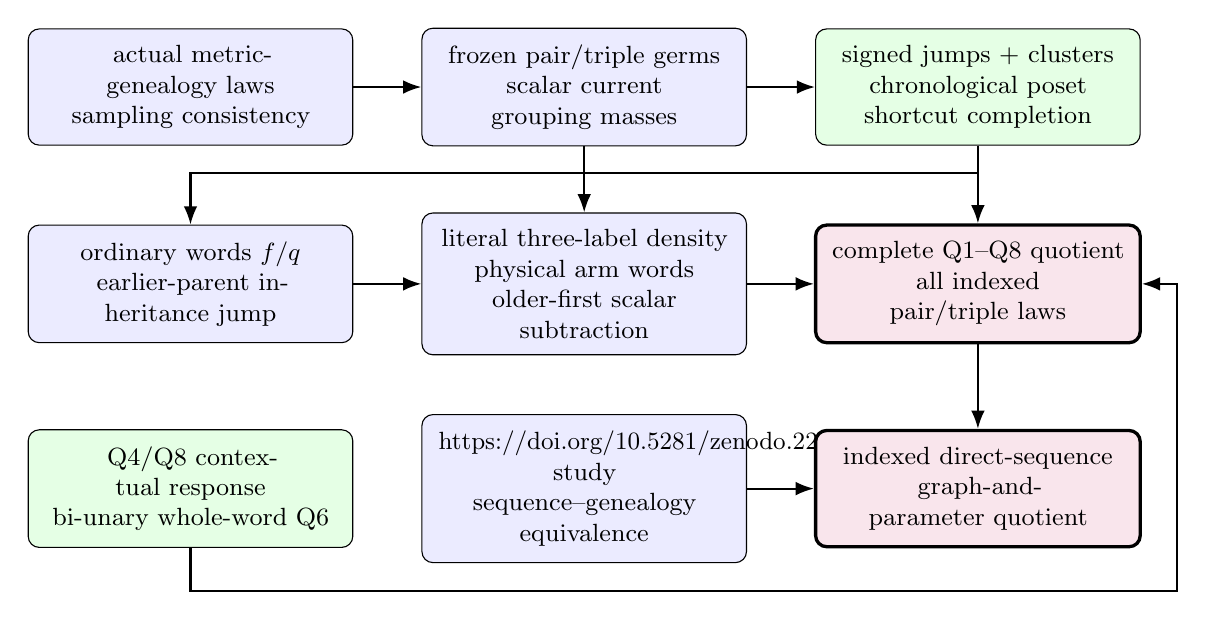
\begin{tikzpicture}[>=Latex,
 box/.style={draw,rounded corners,align=center,text width=3.7cm,minimum height=1.0cm,font=\small,inner sep=6pt},
 observed/.style={box,fill=blue!8}, graph/.style={box,fill=green!10}, final/.style={box,fill=purple!10,very thick}]
\node[observed] (law) at (0,4) {actual metric-genealogy laws\\sampling consistency};
\node[observed] (q) at (5,4) {frozen pair/triple germs\\scalar current grouping masses};
\node[graph] (top) at (10,4) {signed jumps + clusters\\chronological poset\\shortcut completion};
\node[observed] (ordinary) at (0,1.5) {ordinary words $f/q$\\earlier-parent inheritance jump};
\node[observed] (arms) at (5,1.5) {literal three-label density\\physical arm words\\older-first scalar subtraction};
\node[final] (quotient) at (10,1.5) {complete Q1--Q8 quotient\\all indexed pair/triple laws};
\node[graph] (sound) at (0,-1.1) {Q4/Q8 contextual response\\bi-unary whole-word Q6};
\node[observed] (a) at (5,-1.1) {\href{https://doi.org/10.5281/zenodo.22729537}{Companion study}\\sequence--genealogy equivalence};
\node[final] (seq) at (10,-1.1) {indexed direct-sequence\\graph-and-parameter quotient};
\draw[->,thick] (law)--(q); \draw[->,thick] (q)--(top);
\draw[->,thick] (q.south)--(arms.north);
\draw[->,thick] (top.south) -- ++(0,-.35) -| (ordinary.north);
\draw[->,thick] (ordinary)--(arms); \draw[->,thick] (arms)--(quotient);
\draw[->,thick] (top)--(quotient);
\draw[->,thick] (sound.south) -- ++(0,-.55) -| ([xshift=.45cm]quotient.east) -- (quotient.east);
\draw[->,thick] (quotient)--(seq); \draw[->,thick] (a)--(seq);
\end{tikzpicture}}\end{center}
\begin{center}\small All indexed pair/triple laws determine one common graph and its retained parameters. Finite checks support the proofs at their declared scopes.\end{center}
\end{document}
